% Copyright (C) 2012 Shi.Zhan <g.shizhan.g@gmail.com>
%
% Permission is hereby granted, free of charge, to any person obtaining a copy of this software and associated documentation files (the "Software"), to deal in the Software without restriction, including without limitation the rights to use, copy, modify, merge, publish, distribute, sublicense, and/or sell copies of the Software, and to permit persons to whom the Software is furnished to do so, subject to the following conditions:
%
% The above copyright notice and this permission notice shall be included in all copies or substantial portions of the Software.
%
% THE SOFTWARE IS PROVIDED "AS IS", WITHOUT WARRANTY OF ANY KIND, EXPRESS OR IMPLIED, INCLUDING BUT NOT LIMITED TO THE WARRANTIES OF MERCHANTABILITY, FITNESS FOR A PARTICULAR PURPOSE AND NONINFRINGEMENT. IN NO EVENT SHALL THE AUTHORS OR COPYRIGHT HOLDERS BE LIABLE FOR ANY CLAIM, DAMAGES OR OTHER LIABILITY, WHETHER IN AN ACTION OF CONTRACT, TORT OR OTHERWISE, ARISING FROM, OUT OF OR IN CONNECTION WITH THE SOFTWARE OR THE USE OR OTHER DEALINGS IN THE SOFTWARE.
%
% 课程:人机交互技术及应用
% 班级:传播学1001班
% 课时:40学时,2012年秋季1~10周,每周一、三
% 地点:东九楼D212
% 主页:http://code.google.com/p/hci-course/
% 教师:施展 
% 单位:华中科技大学 武汉光电国家实验室
%
\documentclass{beamer}
\usepackage{fontspec,xunicode,xltxtra,beamerthemesplit}
%\usetheme{Hannover} % White background
\usetheme{Berkeley} % Blue background
\setmainfont[
	BoldFont={WenQuanYi Zen Hei},
	ItalicFont={WenQuanYi Micro Hei}
]{WenQuanYi Micro Hei}
\setsansfont[
	BoldFont={WenQuanYi Zen Hei},
	ItalicFont={WenQuanYi Micro Hei}
]{WenQuanYi Micro Hei}

% 中文环境自动换行
\XeTeXlinebreaklocale "zh"
\XeTeXlinebreakskip = 0pt plus 1pt

% 中文环境修正导航栏
\makeatletter
\def\beamer@linkspace#1{
	\begin{pgfpicture}{0pt}{-1.5pt}{#1}{5.5pt}
		\pgfsetfillopacity{0}
		\pgftext[x=0pt,y=-1.5pt]{.}
		\pgftext[x=#1,y=5.5pt]{.}
	\end{pgfpicture}
}
\makeatother

% diagrams
\usepackage{tikz}
\usetikzlibrary{arrows,shapes}

% full page image
\newcommand{\fullPageImage}[2]{
	{
		\usebackgroundtemplate{\includegraphics[width=\paperwidth, height=\paperheight]{#1}}
		\frame[plain]{#2}
	}
}

\title{人机交互技术}
\author{施展}
\institute{华中科技大学~武汉光电国家实验室}
\date{\today}
\titlegraphic{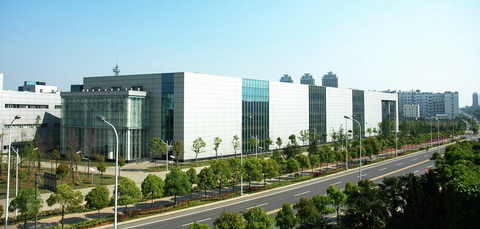
\includegraphics[width=2cm]{images/wnlo.jpg}}

\begin{document}

\begin{frame}
	\titlepage
\end{frame}

\begin{frame}
	\frametitle{内容提要}
	\tableofcontents
\end{frame}

\section{第五讲}
\begin{frame}
	\frametitle{第五讲 界面设计}
	\begin{itemize}
		\item 掌握图形用户界面的主要思想和设计的一般原则。
		\item 了解用户、用户体验、用户交互分析以及设计流程。
		\item 掌握任务分析方法方法
		\begin{itemize}
			\item 重点掌握:使用行为分析、顺序分析、协作关系分析。
		\end{itemize}
		\item 掌握以用户为中心的界面设计方法。
	\end{itemize}
\end{frame}

\subsection{界面设计原则}
\begin{frame}
	\frametitle{界面设计原则}
	\begin{itemize}
		\item 根据表现形式,用户界面分为
		\begin{itemize}
			\item 命令行界面 \textit{Command Line Interface}
			\item 图形界面 \textit{Graphic User Interface}
			\item 多通道用户界面 \textit{Multimodal User Interface}
		\end{itemize}
	\end{itemize}
\end{frame}

\begin{frame}
	\frametitle{图形用户界面的主要思想}
	\begin{itemize}
		\item 图形用户界面的三个重要思想
		\begin{itemize}
			\item 桌面隐喻\\\textit{desktop metaphor}
			\item 所见即所得\\\textit{What You See Is What You Get, WYSIWYG}
			\item 直接操纵\\\textit{Direct manipulation}
		\end{itemize}
	\end{itemize}
\end{frame}

\begin{frame}
	\frametitle{桌面隐喻~\textit{desktop metaphor}}
	\beamertemplatetransparentcovereddynamicmedium
	\begin{beamerboxesrounded}[shadow=true]{桌面隐喻}
		在用户界面中用人们熟悉的桌面上的图例清楚地表示计算机可以处理的能力。
		\begin{itemize}
			\item 图形具有一定的文化和语言独立性,可以提高搜索目标的效率。
			\item 图形用户界面中的图例可以代表对象、动作、属性或其他概念。
		\end{itemize}
	\end{beamerboxesrounded}
	\pause
	\begin{beamerboxesrounded}[shadow=true]{表达方式}
		图例和文字
		\begin{itemize}
			\item 文字适用于表达某些抽象概念。
			\item 图例更易于识别,占用较少屏幕空间,可独立于语言。
		\end{itemize}
	\end{beamerboxesrounded}
\end{frame}

\begin{frame}
	\frametitle{隐喻的表现方法}
	\begin{itemize}
		\item 静态图标
		\item 动画
		\item 视频
	\end{itemize}
\end{frame}

\begin{frame}
	\frametitle{隐喻的分类}
	\begin{itemize}
		\item 直接隐喻:隐喻本身就带有操纵的对象
		\begin{itemize}
			\item 如Word中的表格、图表等图标,图标分别代表了操纵对象。
		\end{itemize}
		\item 工具隐喻:代表所使用的工具
		\begin{itemize}
			\item 如用磁盘图标隐喻存盘操作、用打印机图标隐喻打印操作等,这种隐喻设计简单、形象直观,应用也最为普遍。
		\end{itemize}
		\item 过程隐喻:通过描述操作的过程来暗示该操作
		\begin{itemize}
			\item 如Word中的撤销和恢复图标。
		\end{itemize}
	\end{itemize}
\end{frame}

\fullPageImage{images/RedconsFullPreview1-600x356.png}{\transwipe}

\begin{frame}
	\frametitle{所见即所得}
	\beamertemplatetransparentcovereddynamicmedium
	\begin{itemize}[<+->]
		\item 在WYSIWYG交互界面中显示的用户交互行为与应用程序最终产生的结果是一致的。 
		\item 非WYSIWYG的编辑器,用户只能看到文本的控制代码,对于最后的输出结果缺乏直观的认识。
		\item 思考:孰优孰劣?
	\end{itemize}
\end{frame}

\begin{frame}
	\frametitle{WYSIWYG的弊端}
	\begin{itemize}[<+->]
		\item 平台兼容
		\begin{itemize}
			\item 如果屏幕的空间或颜色的配置方案与硬件设备所提供的配置不一样,在两者之间就很难产生正确的匹配。
		\end{itemize}
		\item 结构隐藏
		\begin{itemize}
			\item 文本处理器都提供了定义章、节、小节等的标记,这些标记显式地标明了对象的属性,但并不是用户最终输出结果的一部分。
		\end{itemize}
	\end{itemize}
\end{frame}

\begin{frame}
	\frametitle{直接操纵}
	\beamertemplatetransparentcovereddynamicmedium
	\begin{beamerboxesrounded}[shadow=true]{直接操纵}
	把操作的对象、属性、关系显式地表示出来,用光笔、鼠标、触摸屏或数据手套等指点设备直接从屏幕上获取形象化命令与数据的过程。
	\end{beamerboxesrounded}
	\pause
	\begin{beamerboxesrounded}[shadow=true]{直接操纵的对象}
	命令、数据或是对数据的某种操作。
	\end{beamerboxesrounded}
\end{frame}

\begin{frame}
	\frametitle{直接操纵的特性}

\end{frame}

\begin{frame}
	\frametitle{直接操纵的优缺点}

\end{frame}

\begin{frame}
	\frametitle{图形用户界面~{\small 一般性原则}}
	\beamertemplatetransparentcovereddynamicmedium
	\begin{itemize}[<+->]
		\item 界面要具有一致性
		\begin{itemize}
			\item 在同一用户界面中,所有的菜单选择、命令输入、数据显示和其他功能应保持风格的一致性。
		\end{itemize}
		\item 常用操作要有快捷方式
		\begin{itemize}
			\item 不仅会提高用户的工作效率,还使界面在功能实现上简洁而高效。
		\end{itemize}
		\item 提供简单的错误处理
		\begin{itemize}
			\item 在出现错误时,系统应该能检测出错误,并且提供简单和容易理解的错误处理功能
		\end{itemize}
		\item 对操作人员的重要操作要有信息反馈
		\begin{itemize}
			\item 尤其是对不常用操作、至关重要操作要有信息反馈。
		\end{itemize}
	\end{itemize}
\end{frame}

\subsection{理解用户}
\begin{frame}
	\frametitle{理解用户}
	\beamertemplatetransparentcovereddynamicmedium
	\begin{itemize}[<+->]
		\item 以用户为中心的设计,宗旨就是:
		\begin{itemize}
			\item 在软件开发过程中要紧紧围绕用户,在系统设计和测试过程中,要有用户的参与,以便及时获得用户的反馈信息;
			\item 根据用户的需求和反馈信息,不断改进设计,直到满足了用户的需求,这个过程才终止。
		\end{itemize}
	\end{itemize}
\end{frame}

\begin{frame}
	\frametitle{所谓“用户”}

\end{frame}

\begin{frame}
	\frametitle{用户体验}

\end{frame}

\begin{frame}
	\frametitle{用户的区别}

\end{frame}

\begin{frame}
	\frametitle{用户交互分析}

\end{frame}

\subsection{设计流程}
\begin{frame}
	\frametitle{设计流程}
	\begin{tikzpicture}[node distance=0.5cm, auto,]
		\node[punkt] (a) {用户的观察和分析};
		\node[punkt, right=of a] (b) {设计};
		\node[punkt, right=of b] (c) {实施};
		\path[line]	(a)--(b);
		\path[line]	(b)--(c);
	\end{tikzpicture}
\end{frame}

\begin{frame}
	\frametitle{用户的观察和分析}
	\begin{itemize}
		\item 情境访谈 Contextual Interviews\\{\tiny 走进用户的现实环境,尽量了解你的用户的工作方式、生活环境等情况。}
		\item 焦点小组 Focus Groups\\{\tiny 组织一组用户进行讨论,让你更了解用户的理解、想法、态度和需求。}
		\item 单独访谈 Individual Interviews\\{\tiny 一对一的用户讨论,让你了解某个用户是如何工作,使你知道用户的感受、想要什么及其经历等。}
	\end{itemize}
\end{frame}

\begin{frame}
	\frametitle{设计}
	\begin{itemize}
		\item 对象模型化: \\{\tiny 将用户分析的结果按照讨论的对象进行分类整理,并且以各种图示的方法描述其属性、行为和关系。}
		\item 低真视图 Low-fidelity Prototype\\{\tiny 比较抽象的视图有利于进行逻辑分析。}
		\item 高真视图 High-fidelity Prototype\\{\tiny 比较具体的视图更接近于人机界面的最终表达。}
	\end{itemize}
\end{frame}

\begin{frame}
	\frametitle{实施}
	\begin{itemize}
		\item 设计师对高真设计原型进行最后的调整,并且撰写产品的设计风格标准(Style Guide),产品各个部分风格的一致性由该标准保证。
		\item 产品实施或投入市场后,面向用户的设计并没有结束,而是要进一步的搜集用户的评价和建议,以利于下一代产品的开发和研制。
	\end{itemize}
\end{frame}

\subsection{任务分析}
\begin{frame}
	\frametitle{任务分析}

\end{frame}

\subsection{以用户为中心的界面设计}
\begin{frame}
	\frametitle{以用户为中心的界面设计}

\end{frame}

\section{小结}
\begin{frame}
	\frametitle{小结}
	\begin{itemize}
		\item 理解人机界面设计的一般原则
		\item 掌握以用户为中心的界面设计方法
	\end{itemize}
\end{frame}

\begin{frame}
	\frametitle{参考文献}
	\bibliographystyle{plain}
	\bibliography{hci}
\end{frame}

\end{document}